\documentclass{sigchi-ext}
% Please be sure that you have the dependencies (i.e., additional
% LaTeX packages) to compile this example.
\usepackage[T1]{fontenc}
\usepackage{textcomp}
\usepackage[scaled=.92]{helvet} % for proper fonts
\usepackage{graphicx} % for EPS use the graphics package instead
\usepackage{balance}  % for useful for balancing the last columns
\usepackage{booktabs} % for pretty table rules
\usepackage{ccicons}  % for Creative Commons citation icons
\usepackage{ragged2e} % for tighter hyphenation

% Some optional stuff you might like/need.
% \usepackage{marginnote} 
% \usepackage[shortlabels]{enumitem}
% \usepackage{paralist}
% \usepackage[utf8]{inputenc} % for a UTF8 editor only

%% EXAMPLE BEGIN -- HOW TO OVERRIDE THE DEFAULT COPYRIGHT STRIP --
% \copyrightinfo{Permission to make digital or hard copies of all or
% part of this work for personal or classroom use is granted without
% fee provided that copies are not made or distributed for profit or
% commercial advantage and that copies bear this notice and the full
% citation on the first page. Copyrights for components of this work
% owned by others than ACM must be honored. Abstracting with credit is
% permitted. To copy otherwise, or republish, to post on servers or to
% redistribute to lists, requires prior specific permission and/or a
% fee. Request permissions from permissions@acm.org.\\
% {\emph{CHI'14}}, April 26--May 1, 2014, Toronto, Canada. \\
% Copyright \copyright~2014 ACM ISBN/14/04...\$15.00. \\
% DOI string from ACM form confirmation}
%% EXAMPLE END

\copyrightinfo{Permission to make digital or hard copies of all or part of this
  work for personal or classroom use is granted without fee provided that
  copies are not made or distributed for profit or commercial advantage and
  that copies bear this notice and the full citation on the first page.
  Copyrights for components of this work owned by others than ACM must be
  honored. Abstracting with credit is permitted. To copy otherwise, or
  republish, to post on servers or to redistribute to lists, requires prior
  specific permission and/or a fee. Request permissions from
  permissions@acm.org.}

% Paper metadata (use plain text, for PDF inclusion and later
% re-using, if desired).  Use \emtpyauthor when submitting for review
% so you remain anonymous.
\def\plaintitle{Ritchie the DeskBuddy: 3D Printed Robot Avatar for Event Reminding}
\def\plainauthor{}
\def\emptyauthor{}
\def\plainkeywords{Ambient Device; Tangible Interface; Personification; 3D Printed Robots}
\def\plaingeneralterms{Documentation, Standardization}

\title{Ritchie the DeskBuddy: 3D Printed Robot Avatar for Event Reminding}

\numberofauthors{2}
% Notice how author names are alternately typesetted to appear ordered
% in 2-column format; i.e., the first 4 autors on the first column and
% the other 4 auhors on the second column. Actually, it's up to you to
% strictly adhere to this author notation.
\author{%
  \alignauthor{%
    \textbf{Dhananjai Hariharan}\\
    \affaddr{Rochester Institute of\\Technology} \\
    \affaddr{Rochester, NY 14623, USA} \\
    \affaddr{dh1723@rit.edu} }\alignauthor{%
    \textbf{Tiago Justino}\\
    \affaddr{Rochester institute of\\Technology} \\
    \affaddr{Rochester, NY, 14623, USA}\\
    \email{tvj6825@rit.edu} } }

% Make sure hyperref comes last of your loaded packages, to give it a
% fighting chance of not being over-written, since its job is to
% redefine many LaTeX commands.
\definecolor{linkColor}{RGB}{6,125,233}
\hypersetup{%
  pdftitle={\plaintitle},
%  pdfauthor={\plainauthor},
  pdfauthor={\emptyauthor},
  pdfkeywords={\plainkeywords},
  bookmarksnumbered,
  pdfstartview={FitH},
  colorlinks,
  citecolor=black,
  filecolor=black,
  linkcolor=black,
  urlcolor=linkColor,
  breaklinks=true,
}

% \reversemarginpar%

\begin{document}

\maketitle

% Uncomment to disable hyphenation (not recommended)
% https://twitter.com/anjirokhan/status/546046683331973120
\RaggedRight{} 

% Do not change the page size or page settings.
\begin{abstract}
Ritchie The DeskBuddy is a 3D printed robotic tiger that works as an ambient
device for reminding and notifying users about events relevant to their life.
In this project, we attempt a different approach to combine digital information
into a physical object, personified by an avatar. Ritchie is a tiger sitting
on a car which plays a melody while waving the arms, blinking the eyes and
moving around. Through the use of such an ambient device, we seek to be able to
drive user reaction and to also form an emotional bond with the user. We also
aim that such a device can be used to imbibe new habits in users.
\end{abstract}

\keywords{\plainkeywords}

\category{H.5.2}{Information interfaces and presentation}{User Interfaces}

\section{Introduction}

There are a wide variety of resources available to people to keep track of
events and activities, to remind them about these, and to make them more
productive. Two commonly used approaches are: (a) using physical reminders such
as post-it notes and diaries, and (b) using software reminders, such as Google
Keep and Google Calendar. The drawback of using post-it notes or diaries is
that the user is physically constrained. That is, if the user has the post-it
notes at home, these notes aren't accessible when they are away from home. On
the other hand, while tools such as Google Keep and Google Calendar are
available to use for free, these are easy to ignore as they only exist
virtually (only provide simple notifications) and are not reflected
sufficiently enough in the physical world.

This project attempts a new approach to providing event reminders. What if it
were possible for a physical object in a user's space to draw attention and
spark user reaction in a more effective manner? What if there could be an
object that can play the role of a friend that reminds you about the occurrence
of an event? Wouldn't it be great if someone were to tell you to stop whatever
you were doing and keep up with your new year's resolution of running a 5K
everyday? Graphical User Interfaces, by their nature, do not create an
emotional bond with a user in most interfaces. Having an emotional bond with an
object can greatly enhance user experience with that particular object,
irrespective of the simplicity of its purpose.

Ritchie the DeskBuddy is just the device for the role. Ritchie is a 3D printed
robotic tiger that sits on a user's desk and reminds them of events or
activities that need to be done. As an internet-connected device, Ritchie can
be of great utility when provided with pertinent data sources, such as Google
Calendar. To be clear, Ritchie is not an AI (Artificially Intelligent) robot.
It cannot tell you what you need to do, or tell you about the weather i.e.\ it
cannot speak. Nor can it specifically remind you to buy some eggs on your way
back home. What Ritchie can do is wave its arms and move around to get your
attention about something important. This should trigger the user to check the
source of this action. The events can range anything from small everyday events
to more important things that demand immediate action.

\section{Related Work}

Peek et.\ al \cite{peek2009hangsters} describe \textit{Hangster}, an ambient
display that embodies virtual interactions using physical devices hanging on
strings. These devices are designed to look like personalized avatars.
\textit{Hangster} allows a person to see their friend's status (online/offline)
on a messaging application (by lowering/raising the avatar), and allow some
simple interactions - e.g.\ initiate a conversation by gently tugging on the
avatar string, show notifications by moving. \textit{Dino}\footnote{Dino -
  Ambient Display Creature: \url{https://www.youtube.com/watch?v=AvST9wjrkC4}} is an
ambient display that controls a physical object to react to the nature of
conversations on a chat application. By studying the content of the
conversation, the `egg' moves to show whether it is happy, sad, angry or calm.
Similarly, \textit{Availabot}\footnote{Availabot:
\url{https://www.youtube.com/watch?v=w0voYnEjFcQ}} is a computer-controlled push
puppet that stands or falls down to reflect a friend's availability
(online/offline status) on a chat application.

Jafarinaimi et.\ al \cite{jafarinaimi2005breakaway} describe
\textit{Breakaway}, an ambient display that attempts to encourage people who
sit for long periods to take more frequent breaks. This is implemented using a
shape-changing artistic sculpture object. User's position and posture is
tracked using various sensors. Shape and movement of the device reflects the
user's pose - upright when the user takes a break, and slouching when the
person has been sitting for extended periods. Similar to \textit{Breakaway},
\textit{MoveLamp} \cite{fortmann2013make} keeps track of a person's physical
activity at the workplace and attempts to encourage physical activity when a
person has been sitting for long periods. This made use of a pedometer
application on a smartphone, in combination with software on a computer to
control an ambient lamp that changed color from green to red to make the user
aware that they need to move. Rogers et.\ al \cite{rogers2010ambient}
investigated whether ambient displays can be used to influence behavioral
changes among people. In this study, they installed twinkly lights in the
carpets to unconsciously guide people to take the stairs. A large ambient
display in the common area was used to visualize the number of people using the
stairs vs.\ those that chose to use the elevator. While each of these were
implemented differently, they shared a common goal of nudging a user towards an
action and observing common behavioral changes over extended periods of time.

In \textit{Tangible Bits} \cite{ishii1997tangible}, Hiroshi Ishii proposes the
concept of coupling the digital world (bits of information) into a physical
object, thereby making it `tangible'. In line with this concept, Ritchie The
DeskBuddy would be a Tangible Bit, where the object would mirror digital
information and events, acting as a `phicon', or a physical icon.
\textit{ReaDIYmate}\footnote{ReaDIYmate: \url{http://readiymate.com/}} is a
commercially available DIY (Do-It-Yourself) kit for building internet-connected
paper objects that react to events in the digital world.  Similarly, few other
devices exist that physically react to digital events and interactions -
\textit{Olly}\footnote{Olly: \url{http://www.ollyfactory.com/}} is a device that
releases a scent for certain digital events/interactions. Similarly,
\textit{Polly}\footnote{Polly project: \url{http://www.ollyfactory.com/polly/}} is a
device that releases a ball of candy for certain digital events/interactions.

%\begin{marginfigure}[-35pc]
%  \begin{minipage}{\marginparwidth}
%    \centering
%    \includegraphics[width=0.9\marginparwidth]{../photos/android}
%    \caption{Android toy that will be used to inspire Ritchie's design.}
%    \label{fig:android}
%  \end{minipage}
%\end{marginfigure}

Besides the above mentioned research and projects, there is sufficient work in
the area of 3D printed robots and robot parts\cite{megaro2015interactive,
schulz2015interactive}\footnote{Instructables page: ``GearBot: A Dual-speed,
Gear-driven robot'':
\url{http://www.instructables.com/id/GearBot-A-Dual-Speed-Gear-Driven-Bot/?ALLSTEPS}}\footnote{Cubify
- Commercial 3D printed parts for custom designed robots:
\url{http://cubify.com/store/mrn}}, as well as numerous resources for accessing 3D
models of robots and parts for 3D printing.

\section{Project Description}

Ritchie The DeskBuddy is a 3D printed robotic tiger that sits on a user's desk
and reminds them of events or activities that need to be done.

\subsection{Information Displayed}

The device reflects reminders, events and tasks relevant to a user. The same
concept can be used to developing and practicing some new habits as well, e.g.\
reading one chapter of a book everyday, running 5K, practice sketching etc.

\subsection{Data Source}

For this project, Google Calendar\footnote{Google Calendar API:
  \url{https://developers.google.com/google-apps/calendar/}} was used as the data
source, as it is already widely used by many users as an application for
recording activities and keeping track of events.

\subsection{Device Components}

The following components were used to build Ritchie the DeskBuddy:

\begin{itemize}
  \item Particle Photon;
  \item 1200mAh Lithium battery;
  \item Photon battery shield;
  \item Continuous Rotation Micro Servo;
  \item 180deg rotation Micro Servo;
  \item Accelerometer;
  \item Piezoelectric speaker;
  \item White LED.
\end{itemize}

\subsection{Device abilities}

The 3D printed robot will be able to do the following:
\begin{itemize}
  \item Perform a waving action (arm movement);
  \item Move on a flat surface (walk/drive);
  \item Play certain sounds for certain events;
  \item Blink lights to attract attention.
\end{itemize}

\subsection{Mapping of information to visualization}

The basic device capabilities are:

\begin{itemize}
  \item Perform a waving action (arm movement):

    The waving arms are controlled using a micro servo motor. The motor pulls a
    string that connects both the arms of the robot. By alternately pulling and
    releasing the string, the arms are raised and dropped. Using this
    mechanism, it is possible to create the waving action in the robot. The
    visual effect can be seen on Figure~\ref{fig:arms}.

\begin{figure}
  \includegraphics[width=0.9\columnwidth]{../photos/arms}
  \caption{Arm-waving movement produced by pulling a string with a
    servo.}~\label{fig:arms}
\end{figure}

\item Move forward/backward:

  The robot uses wheels to move. The forward/backward motion of the robot is
  performed using a continuous rotation motor, which is used for turning one of
  the wheels. This is done by creating spokes on one of the wheels, which can
  be pushed by the rotation motor. Figure~\ref{fig:motor} shows the mechanism
  used for producing the movement.

\begin{figure}
  \includegraphics[width=0.9\columnwidth]{../photos/motor}
  \caption{Motor used to move the wheel with spokes.}~\label{fig:motor}
\end{figure}

\item Play certain sounds for certain events:

  The robot uses a piezoelectric speaker to play melodies during the
  event-reminding action.

\item Blink lights to attract attention:

  A white LED is used to light the robot eyes, again, to attract the user's
  attention.

\end{itemize}


\subsection{Design}

All the parts for 3D printing were modelled using TinkerCad\footnote{TinkerCad:
  \url{https://www.tinkercad.com/}}. The tiger head for the robot was created by
removing the unwanted parts of a Tiger model\footnote{Tiger model available on
  TinkerCad: \url{https://www.tinkercad.com/things/fhidfq2ZhEC-tiger}} available for
use on the TinkerCad gallery. By modifying this model, it was possible to make
the head hollow in order to house the LED and the piezo speaker, as well as
create eye sockets. Figure~\ref{fig:head} shows the resulting 3D printed head.

\begin{figure}
  \includegraphics[width=0.9\columnwidth]{../photos/head}
  \caption{3D printed from modified tiger model.}~\label{fig:head}
\end{figure}

The main body of the robot was designed to house the head, the arms, as well as
cover some of the electronics at the base. Together with a back case designed
to look like a jetpack, these parts cover most of the electronics in the robot.
The ``jetpack'' case mainly hides the big motor, the micro servo and the battery.
The photon, the battery shield and most of the wires are hidden under the
tiger. Figure~\ref{fig:jetpack} shows the back case and the battery attached to
it and Figure~\ref{fig:body} shows the main body.

\begin{figure}
  \includegraphics[width=0.9\columnwidth]{../photos/jetpack}
  \caption{Back case designed as a jet pack (left) holding the battery (right).}~\label{fig:jetpack}
\end{figure}

\begin{figure}
  \centering
  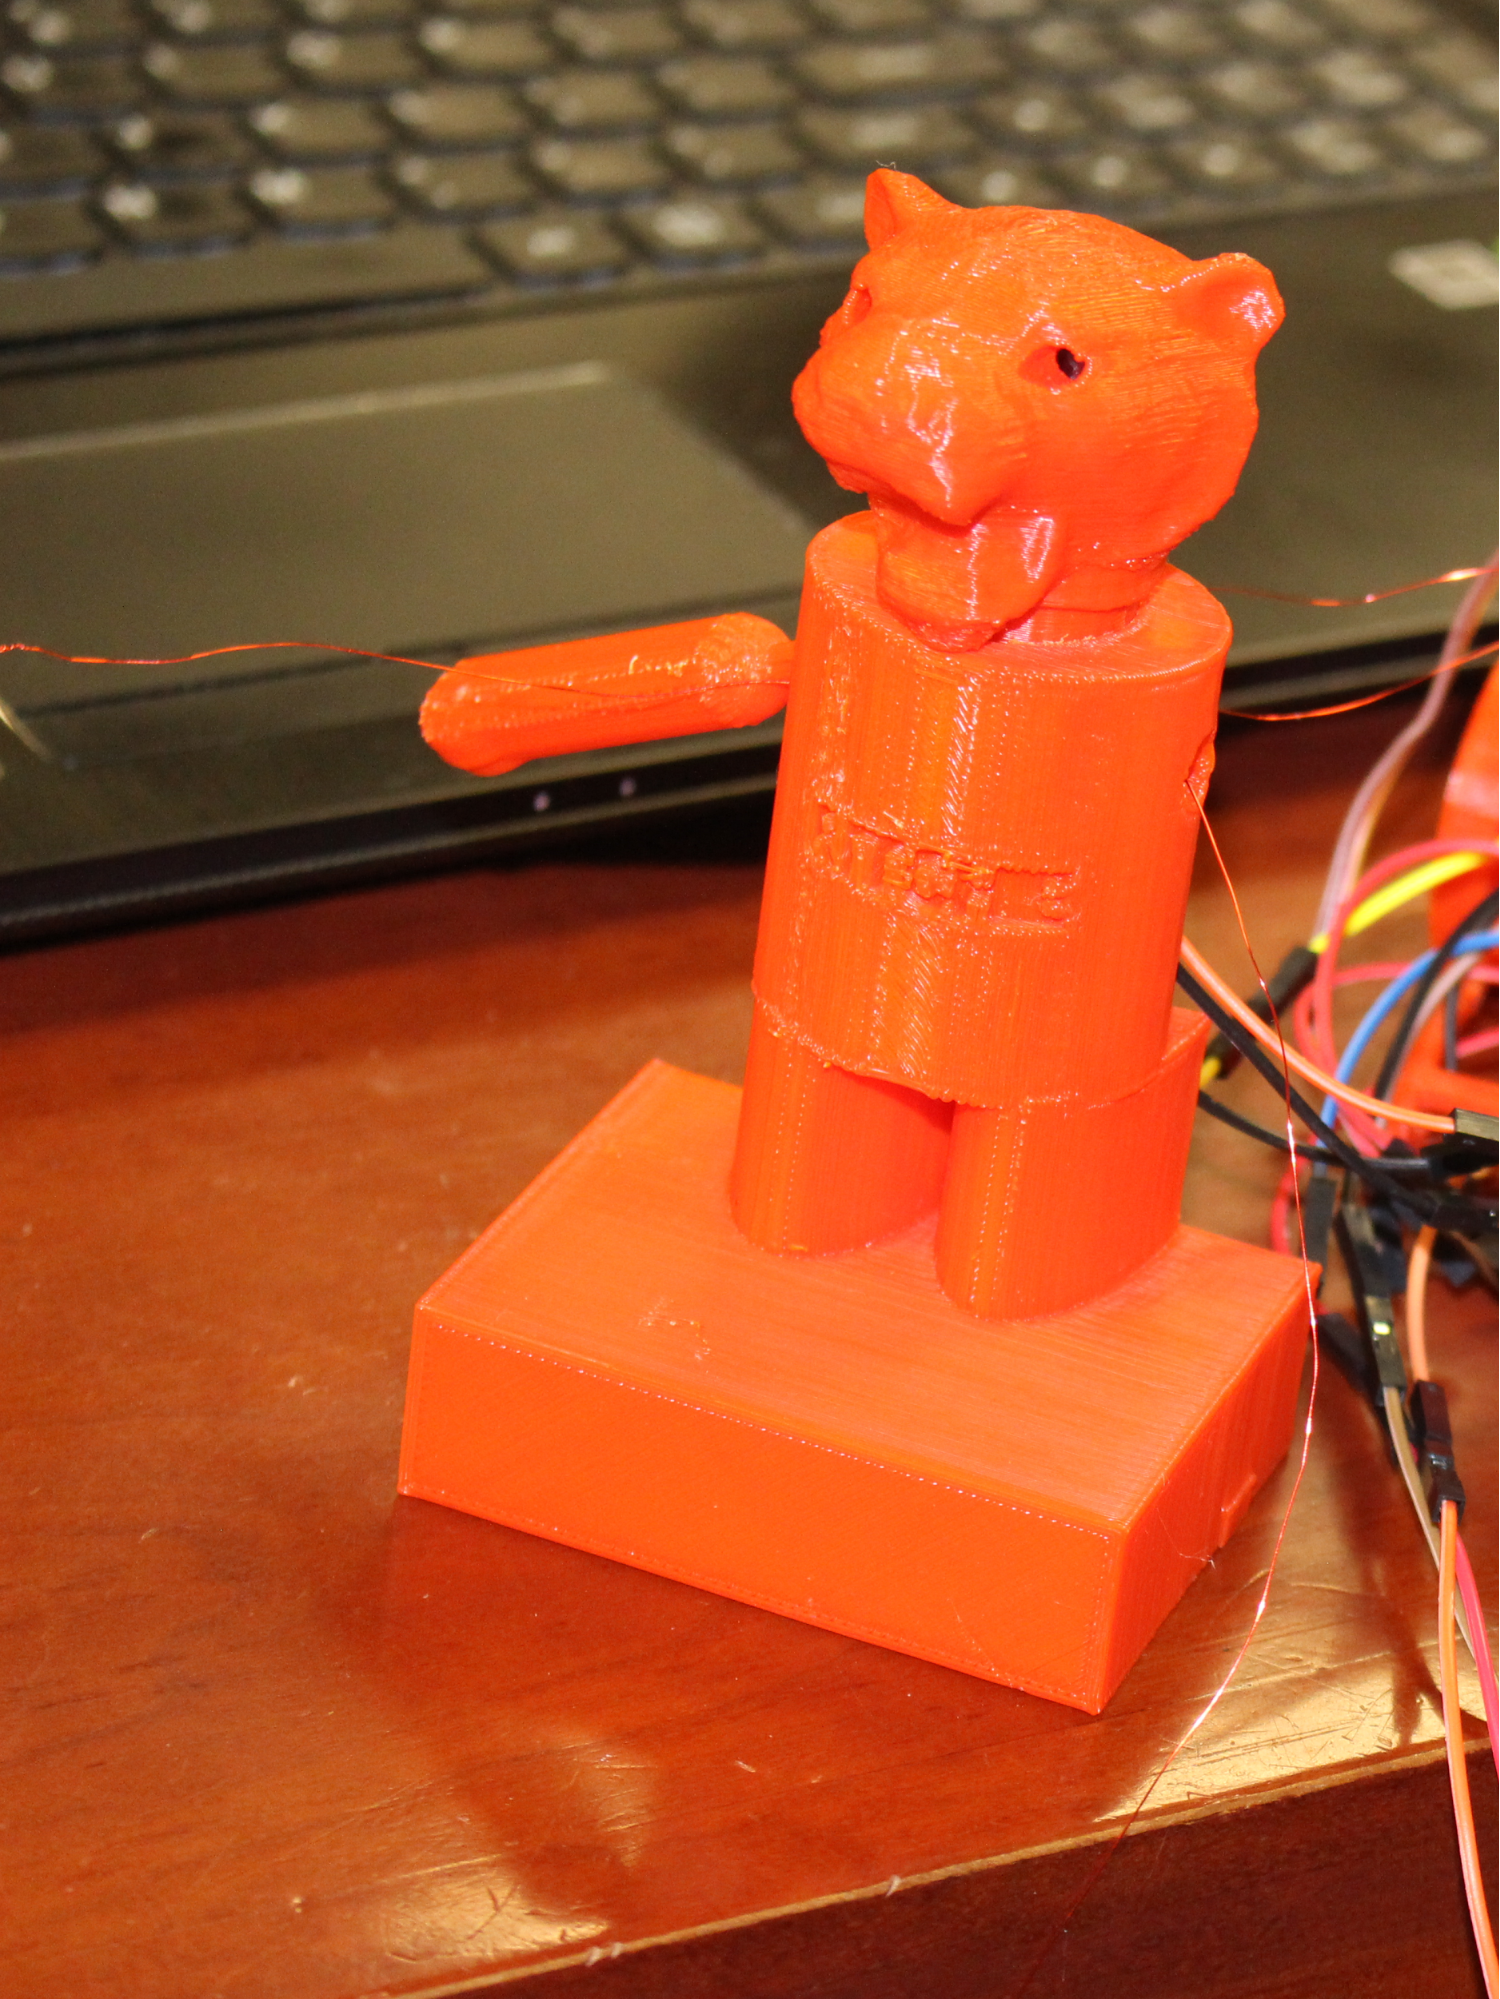
\includegraphics[width=0.5\columnwidth]{../photos/body}
  \caption{Main body with head and right arm.}~\label{fig:body}
\end{figure}
%\begin{marginfigure}[-35pc]
%  \begin{minipage}{\marginparwidth}
%    \centering
%    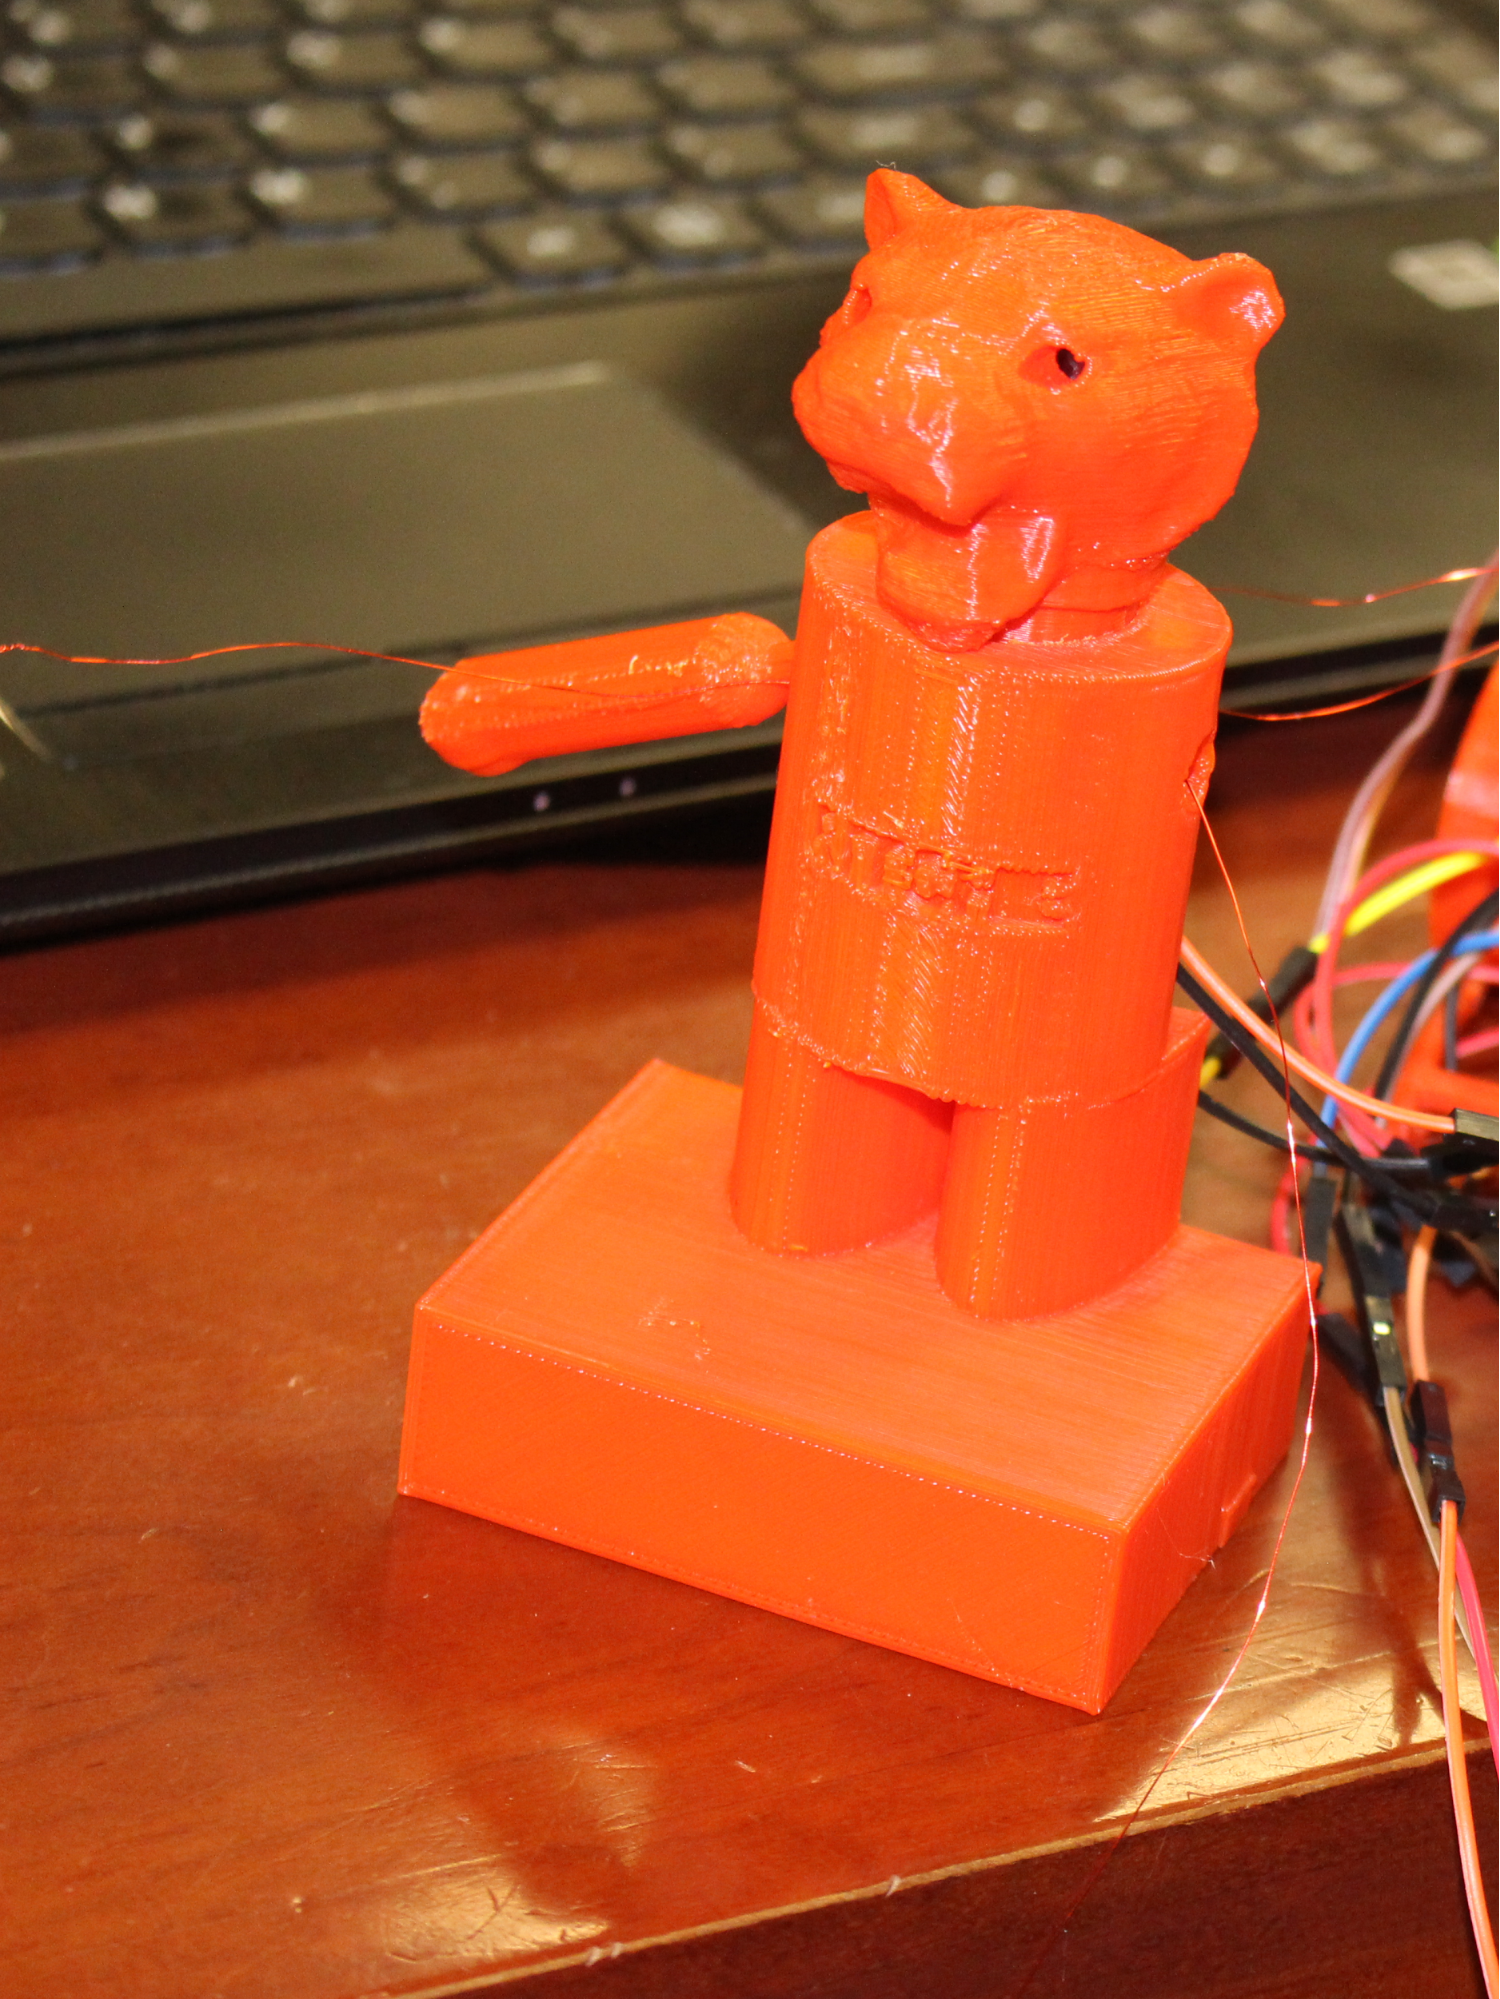
\includegraphics[width=0.9\marginparwidth]{../photos/body}
%    \caption{Main body with head and right arm.}
%    \label{fig:body}
%  \end{minipage}
%\end{marginfigure}

The base of the device holds the four wheels which allows the robot to move. As
mentioned above, one of the wheels is designed differently so that it can be
controlled using the continuous rotation servo. Figure~\ref{fig:photon} shows
the base holding together the wheels, the battery shield and the photon.
Lastly, Figure~\ref{fig:final} shows the final assembled device.

\begin{figure}
  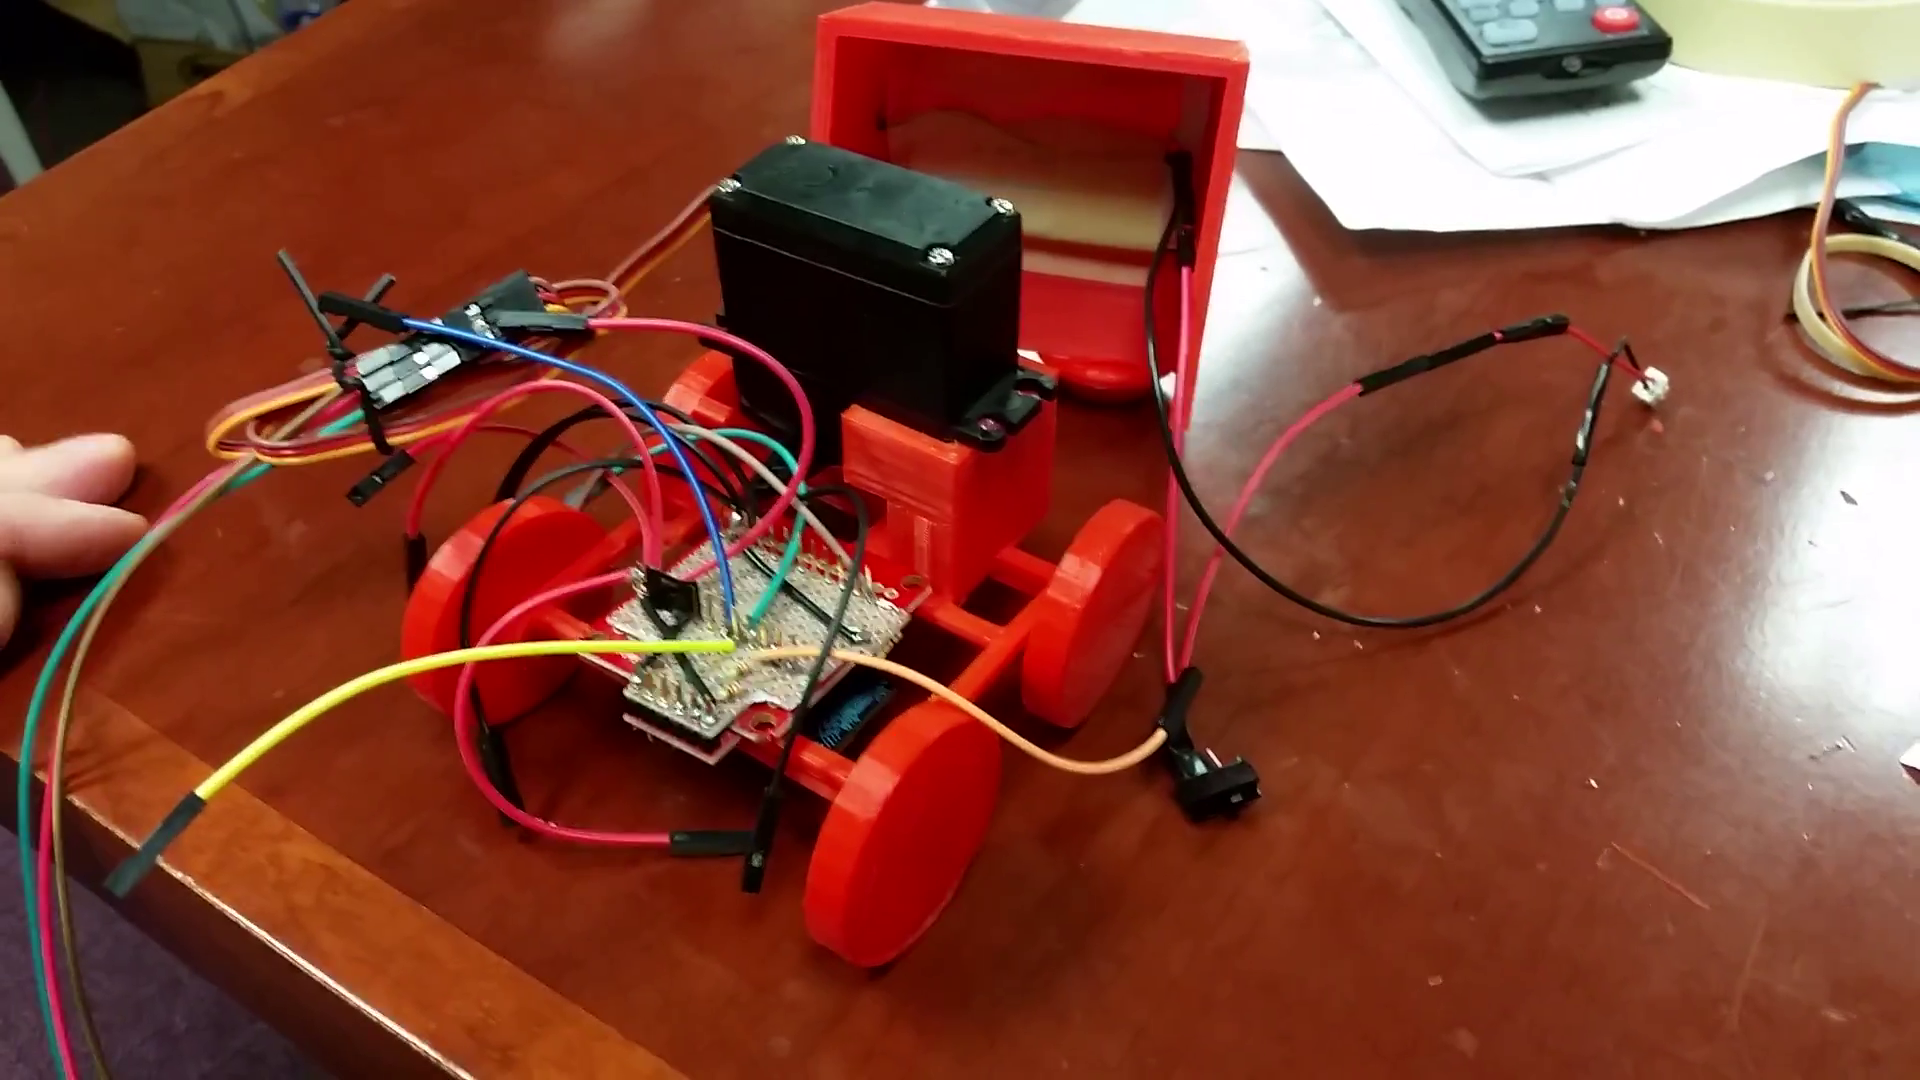
\includegraphics[width=0.9\columnwidth]{../photos/photon}
  \caption{Wheels with photon and battery shield.}
  \label{fig:photon}
\end{figure}

\begin{figure}
  \includegraphics[width=0.9\columnwidth]{../photos/final}
  \caption{Final assembled product.}
  \label{fig:final}
\end{figure}

\subsection{Events and Information Visualization}

The current implemented system displays 5 different types of events, with
different priorities, using various combinations of the actions described
above. The actions for each of the events are specific to each category. In
order to identify the various events, we make use of the color tags in Google
Calendar, which can be assigned to different events. For each event in the
calendar, the only details that are needed by the device are the event color
(colorID), and the event start and end time.

Since there are various priority levels involved, it is also important to
ensure that higher priority events do not get overlooked as lower priority
events in the case of event concurrency. For example, an ``Important'' event
could be overlooked as a ``regular'' event if the robot performs the action for
a regular event. We tackled this by checking for concurrent events, so that we
ensure that the device behaves respective to the highest priority concurrent
event. The actions for each event type are described as follow:

\subsubsection{Important Events}

``Important'' events are flagged BOLD RED in the Calendar. The robot displays
these events by waving its arms at a preset ``high'' frequency as well as by
moving back and forth at a fast speed. These physical actions are accompanied
by flashing the lights in the robot's eyes and by playing the Shave and a
Haircut\footnote{Shave and a Haircut, two bits:
  \url{https://en.wikipedia.org/wiki/Shave\_and\_a\_Haircut}} melody specific for this
category.

\subsubsection{Alarms}

``Alarm'' events are flagged YELLOW in the Calendar. The robot sounds an alarm by
playing some preset music. In this implementation, we play the ``Nyan Cat''
theme song\footnote{Playing ``Nyan Cat'' on Arduino:
  \url{http://www.instructables.com/id/Nyan-Cat-on-Arduino/}}. 

\subsubsection{Workout}

Since one of the goals of this project is to help users develop new habits, we
selected ``working out'' / ``going to the gym'' as one of the special use cases of
this feature. ``Workout'' events are flagged GREY in the Calendar. This is
visualized by the robot waving it's arms at a preset ``medium'' speed, as well as
by moving back and forth at a slower speed as compared to the ``important''
events. The robot also flashes its eyes using the LED and plays some music. For
the music, we chose to play ``Eye of the Tiger''\footnote{Playing ``Eye of the
  Tiger on Arduino: \url{http://forum.arduino.cc/index.php?topic=215687.0}} as something that would be
motivational and encourage the user to workout.

\subsubsection{Activity/Habit slots}

The ``Workout'' and ``Alarm'' conditions are special use cases of this type of
event. Users can flag their events PURPLE if they wish to save time for
activities such as reading a book, writing a diary etc. These events are
represented in the same manner as the ``workout'' condition. In this condition,
the robot plays the ``Gonna Fly Now'' theme\footnote{Playing ``Gonna Fly Now''
  on Arduino:
  \url{http://mleighsmith.tumblr.com/post/116526557727/chill-out-pump-up}}.

\subsubsection{Regular Events}

``Regular'' events are simply other events from the user's Calendar, but do not
require a special action. All colors not used by the above events are
considered as ``Regular'' events. At the start of the event, the robot makes a
short beeping sound, and then waves it arms for a short duration. The arm
motion is at a slower frequency as compared to the ``Activity'' event.

All of the above mentioned device actions occur at the start of an event. For
the duration of an event, the robot repeats some of the actions at intervals
(we have set this interval at 15 minutes), to represent ongoing events. This also
meant to act as an ambient reminder. As mentioned above, the robot also moves
for some events. This motion is always a preset distance, however, the speed
and frequency with which it moves varies for different conditions.

In it's default state, the device does not perform any actions and waits to
receive information for the next event.

\subsection{User Interaction}

By using an accelerometer, the robot can afford some simple user interactions
such as ``Tap'' and ``Shake'' gestures. Tap gestures can be used to snooze event
reminders from the robot. Once snoozed, the reminder occurs again after 15
minutes. Reminders can be completely blocked for the duration of the event
using a shake gesture. Each user interaction is acknowledged using a beeping
sound.

Additionally, the robot can be put in a ``Do Not Disturb'' mode, by placing it
on it's side. In this orientation, the device will deactivate and no event
actions will occur. Figure~\ref{fig:dontdisturb} shows Ritchie on the ``Do Not
Disturb'' position. As a fun addition to the device features, the user can
trigger the Nyan Cat music to play by vigorously shaking the device.

\begin{figure}
  \includegraphics[width=0.9\columnwidth]{../photos/dontdisturb}
  \caption{Ritchie placed on ``Do Not Disturb'' position.}
  \label{fig:dontdisturb}
\end{figure}

\section{Observations}

The first observation from the end-result of this project would be that the
robot was much bigger than we had initially imagined. Figure~\ref{fig:size} is
compares the scale of the robot with other toys that would ideally
perform actions such as our proposed device.

\begin{figure}
  \includegraphics[width=0.9\columnwidth]{../photos/size}
  \caption{Ritchie with other toys for size comparison}
  \label{fig:size}
\end{figure}

The waving-arm motion was not as smooth and exaggerated as initially planned.
The mechanism for the arms were planned such that there would be a large arm
motion (i.e.\ the arm motion would span a larger angle).

The flashing lights in the head of the robot are not very bright. This is due
to the fact that only one LED was used, which is placed in the center of the
head. Also, the holes for the eye sockets are at varying depths, due to the
uneven shape of the head model. This causes the light to appear brighter in one
eye. We attempted to use aluminum foil inside the head to reflect and amplify
the light, but we observed only a marginal improvement.

The micro servo motor, used for controlling the arms, makes a lot much noise.
In a way, this is a good thing because this catches the user's attention well.
At the same time, this is a negative effect as it clashes with the music and
tones played by the speaker.

\section{Challenges \& Limitations}

This project was not short on challenges and every phase of development
presented us with interesting obstacles and difficulties. This project
encountered all the challenges associated with 3D printing and prototyping - 3D
modelling, getting all the object dimensions right and ensuring that all the
various parts fit together. Another major challenge was to plan the design
before hand, keeping the accommodation of all the electronic components in
mind.

As mentioned in the previous section, the final robot was much larger than
initially imagined. This was largely down to the use of the continuous rotation
servo for moving the robot, which is very big in size. Barring this part, the
robot could have been designed to be reasonably smaller.

We observed that the shaking interaction requires a sturdy model, both within
and without. Our current model has various separate 3D printed parts, which
need to hold together well. Inside the robot some parts, such as the thinner
wires broke several times during testing, which is not ideal. It is also really
difficult to keep everything (the Particle Photon, the battery shield, battery,
piezo speaker, LED, motors and wires) inside the robot, and at the same time
have a reasonable size for good user interaction.

We encountered some difficulty with implementing the ``tap'' detection with our
robot. Individually, tap detection using the accelerometer is quite simple as
this is managed by a library\footnote{MMA8452Q Accelerometer library:
  \url{https://github.com/sparkfun/MMA8452\_Accelerometer}}. However, tap detection in
the fully-functioning robot was really tricky - we found that the arm movement
would trigger the ``tap'' function due to the vibrations that it caused. After
extensive testing and experimentation, we managed to modify the threshold such
that the device would ignore the jolts from the micro servo, yet at the same
time reliably detect the tap gestures.

As mentioned in the previous section, the LED lights through the eyes were not
as visible as we would have preferred. Although we attempted to use aluminum
foil inside the head to reflect and brighten the light, we did not notice any
significant improvement.

\section{Conclusion \& Future Work}

The proposed project to build a 3D printed robotic tiger was successfully
executed. 3D printing was employed for creating all the parts of the robot. We
succeeded in connecting the robot with user data in Google Calendar and produce
the desired actions. The robot is capable of representing up to 5 different
types of events. The robot allows for user interaction using tapping and
shaking.

Despite having successfully executing and implementing the project as per the
initial proposal, there is a lot of scope for improvement. In the future, the
design for the robot can be improved to ensure that all the electronics
components and all wires are completely encased and tucked inside the device.
The current design has a gap between the robot and the jetpack which is open
and exposes the electronics to some extent. Since this is a working prototype,
having that gap helps us monitor the functioning of the various components and
fix problems.

We would also like to make the overall device smaller and more compact. We
could also create an interface to allow users to customize the robot behavior
to their desire within a limited set of parameters (movement speed, movement
length, led blinking pattern, melody selection, arm waving frequency etc.) as
well as integrate with other services like Gmail, Twitter and Facebook.

It would also be interesting to conduct a study and observe user employment of
such an ambient device. Some research questions would be - Do users find it
useful to have such an ambient device to provide them with relevant digital
information? Does this device make its user more productive? Would users use
this robot to set the practice of engaging in new habits such as keeping fit or
reading a book? Is such a system an effective method for affecting user
behavior? The results of such a study would provide insight into the use of
ubiquitous devices for having a positive effect on user behavior.

%\marginpar{%
%  \vspace{-45pt} \fbox{%
%    \begin{minipage}{0.925\marginparwidth}
%      \textbf{Good Utilization of the Side Bar} \\
%      \vspace{1pc} \textbf{Preparation:} Do not change the margin
%      dimensions and do not flow the margin text to the
%      next page. \\
%      \vspace{1pc} \textbf{Materials:} The margin box must not intrude
%      or overflow into the header or the footer, or the gutter space
%      between the margin paragraph and the main left column. The text
%      in this text box should remain the same size as the body
%      text. Use the \texttt{{\textbackslash}vspace{}} command to set
%      the margin
%      note's position. \\
%      \vspace{1pc} \textbf{Images \& Figures:} Practically anything
%      can be put in the margin if it fits. Use the
%      \texttt{{\textbackslash}marginparwidth} constant to set the
%      width of the figure, table, minipage, or whatever you are trying
%      to fit in this skinny space.
%    \end{minipage}}\label{sec:sidebar} }

%\begin{figure}
%  \includegraphics[width=0.9\columnwidth]{figures/sigchi-logo}
%  \caption{Insert a caption below each figure.}~\label{fig:sample}
%\end{figure}

% \begin{figure}
%   \includegraphics[width=.9\columnwidth]{figures/ea-figure2}
%   \caption{If your figure has a light background, you can set its
%     outline to light gray, like this, to make a box around
%     it.}\label{fig:bats}
% \end{figure}

%\begin{marginfigure}[-35pc]
%  \begin{minipage}{\marginparwidth}
%    \centering
%    %\includegraphics[width=0.9\marginparwidth]{figures/cats}
%    \caption{In this image, the cats are tessellated within a square
%      frame. Images should also have captions and be within the
%      boundaries of the sidebar on page~\pageref{sec:sidebar}. Photo:
%      \cczero~jofish on Flickr.}~\label{fig:marginfig}
%  \end{minipage}
%\end{marginfigure}

%\begin{figure*}
%  \centering
%  \includegraphics[width=1.4\columnwidth]{figures/map}
%  \caption{In this image, the map maximizes use of space. You can make
%    figures as wide as you need, up to a maximum of the full width of
%    both columns. Note that \LaTeX\ tends to render large figures on a
%    dedicated page. Image: \ccbynd~ayman on Flickr.}~\label{fig:cats}
%\end{figure*}

%\marginpar{\vspace{-23pc}So long as you don't type outside the right
%  margin or bleed into the gutter, it's okay to put annotations over
%  here on the left, too; this annotation is near Hawaii. You'll have
%  to manually align the margin paragraphs to your \LaTeX\ floats using
%  the \texttt{{\textbackslash}vspace{}} command.}

%\begin{margintable}[1pc]
%  \begin{minipage}{\marginparwidth}
%    \centering
%    \begin{tabular}{r r l}
%      & {\small \textbf{First}}
%      & {\small \textbf{Location}} \\
%      \toprule
%      Child & 22.5 & Melbourne \\
%      Adult & 22.0 & Bogot\'a \\
%      \midrule
%      Gene & 22.0 & Palo Alto \\
%      John & 34.5 & Minneapolis \\
%      \bottomrule
%    \end{tabular}
%    \caption{A simple narrow table in the left margin
%      space.}~\label{tab:table2}
%  \end{minipage}
%\end{margintable}

\balance{}

\bibliographystyle{SIGCHI-Reference-Format}
\bibliography{references}

\end{document}

%%% Local Variables:
%%% mode: latex
%%% TeX-master: t
%%% End:
